% 93-28(93쪽) — 서로 외접하는 세 원 A, B, C 와 세 중심을 이은 삼각형 ABC(원문 「오른쪽 그림」). 스캔 화질이 낮아 TikZ 로 다시 그림.
% 라벨은 원문 것만: 세 중심 A·B·C. 넓이의 비·반지름·cos B 의 값(답)은 그림에 적지 않는다.
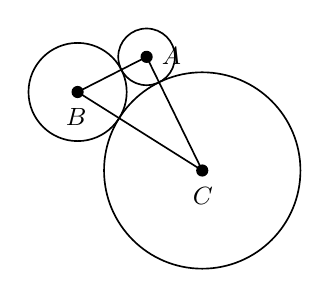
\begin{tikzpicture}[line width=0.6pt, x=0.36cm, y=0.36cm]
  \coordinate (A) at (2.434,1.240);
  \coordinate (B) at (0,0);
  \coordinate (C) at (4.397,-2.769);
  \draw (A) circle [radius=1];
  \draw (B) circle [radius=1.732];
  \draw (C) circle [radius=3.464];
  \draw (A) -- (B) -- (C) -- cycle;
  \fill (A) circle (2.2pt);
  \fill (B) circle (2.2pt);
  \fill (C) circle (2.2pt);
  \node[font=\small, anchor=west] at (2.62,1.26) {$\pt{A}$};
  \node[font=\small, anchor=north] at (-0.05,-0.22) {$\pt{B}$};
  \node[font=\small, anchor=north] at (4.42,-3.00) {$\pt{C}$};
\end{tikzpicture}
